\section{Method}
\label{sec:method}

\subsection{Information-System Architecture and Evidence Boundary}
\label{sec:method_overview}

The system has four layers: query representation, corpus/index retrieval, evidence serialization and audit/evaluation (Figure~\ref{fig:method_pipeline}). Query representation produces a question vector, rewrite, hypothetical passage or iterative query. A frozen dense or BM25 index retrieves records; the serializer passes corpus evidence to a short-answer reader. Evaluation measures completeness, EM/F1, paired uncertainty, calls, content overlap and provenance. Query-composition diagnostics appear in Online Resource 1, Section~\SuppRef{sec:supp_answer_overlap_normalization}.

\begin{figure}[tbp]
\centering
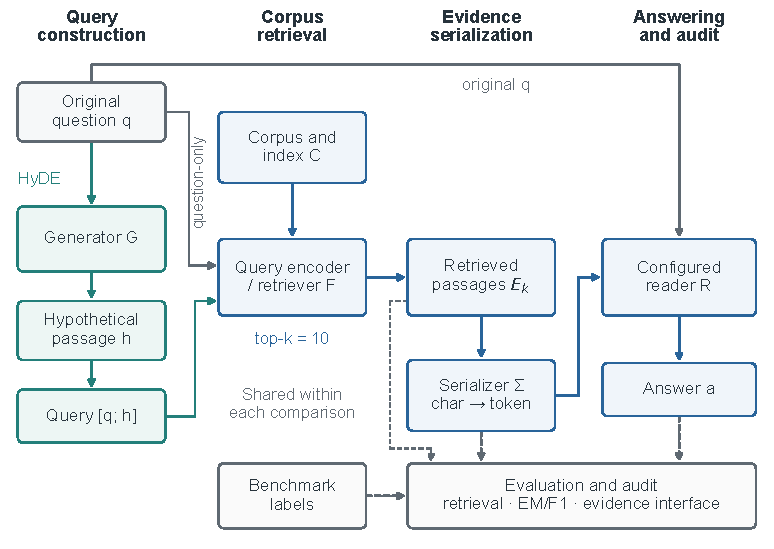
\includegraphics[width=\textwidth]{Fig1_Workflow.pdf}
\caption{System workflow and evidence boundary. Question-only and HyDE are separate conditions sharing the corpus, index, retrieval configuration and top-$k=10$ within each comparison. HyDE forms $[q;h]$ from the question $q$ and hypothetical passage $h$. The reader receives the original question and serialized corpus evidence under condition-specific character and token budgets. Solid arrows show inference; dashed arrows show evaluation and audit. Benchmark labels enter evaluation only. Optional answer postprocessing is omitted.}
\label{fig:method_pipeline}
\end{figure}


The controlled tier uses released candidate pools and a question-independent 100k pool; the HotpotQA full-wiki tier adds iterative retrieval on a 5.23-million-paragraph index. In the primary retrieval tiers, readers see only the original question and retrieved corpus evidence, excluding hypothetical documents, rewritten queries, gold markers and reasoning traces. Supporting-title completeness is primary; exact-record and serialized-evidence coverage are distinct diagnostics. The exploratory guarded answer-format analysis remains secondary (Online Resource 1, Section~\SuppRef{sec:supp_verifier_guard_decomposition}).

The audit identifies each system as $S=(G,F,C,\Sigma,R,B)$: generator, retrieval function, corpus/index, evidence serializer, reader and operating budget. An observed configuration edge carries source/target effects, metric direction, paired intervals, frozen sample identifiers and artifact hashes. Binary local decisions use two-sided exact paired tests with Holm adjustment within the declared family. Favorable significant effects support a local gain; adverse significant effects support its opposite direction. Other local decisions remain unresolved. Reader interactions use separately declared paired sign-flip tests where applicable; intervals estimate uncertainty rather than decide significance.

Transport additionally requires an eligible, favorable source effect with $p_{\mathrm{Holm}}<0.05$. Supported transport requires favorable adjusted decisions for all required target effects; contrary adjusted evidence can reject it, while absent or ineligible evidence leaves it unresolved. Thus a supported local reranker gain need not establish transport from the source configuration. Metrics remain separate, and changing multiple components prevents causal attribution. Table~\ref{tab:boundary_stability_matrix} names local contrasts underlying the overview; the complete CSV retains source-and-target classifications and hashes. This is an empirical audit workflow, not a new retrieval algorithm or statistical test.

\subsection{Formal Protocol and Boundaries}
\label{sec:formal_protocol}

For question $q$ and title--paragraph corpus $\mathcal{C}$, the generator produces $h=G(q)$. The primary dense query is $[q;h]$, ranked by $\mathrm{sim}(f([q;h]),f(d))$ to obtain top-$k$ corpus evidence $E_k$ and answer $a_0=R(q,E_k)$. Question-only, rewrite and hypothetical-only variants are diagnostics. The generated passage is a retrieval representation, not reader evidence; factual correctness and completeness are not guaranteed.

\subsection{Open-Weight Confirmatory Tier}
\label{sec:open_weight_confirmatory_tier}

The two local generators are revision-pinned Qwen2.5-7B-Instruct and Mistral-7B-Instruct-v0.3; revisions and prompts are recorded in Online Resource 1, Section~\SuppRef{supp:sec:open_weight_confirmatory_protocol}. Both use greedy decoding, seed 13 and a 96-token cap. The Qwen tier compares question-only Dense, standard HyDE, evidence-only HyDE and Query2doc-style (4-shot adaptation); deterministic target-dependent demonstration selection is documented in the supplement. Mistral repeats standard HyDE with the same question order, serialization and retrieval settings, without model-specific tuning.

All conditions hold BGE-base at revision \path{a5beb1e3e68b9ab74eb54cfd186867f64f240e1a}, CLS pooling, L2 normalization, a 512-token input limit and top-$k=10$ fixed. Evaluation gold answers and support flags are never supplied to the generator outside the explicitly fixed training demonstrations. This tier measures retrieval only; no reader result is inferred. Sanitized public rows retain stable IDs, condition, rank, document IDs, scores and metric fields while excluding benchmark text and unrestricted generations.

\subsection{Post-Hoc and Pre-Output Sensitivity Analyses}
\label{sec:review_driven_sensitivity}

Four additional sensitivity analyses were specified before inspecting their own outputs, after the initial study; they are not preregistered evidence. Retrospective evidence diagnostics are identified separately. Sample order is fixed; resampling uses seed 13 and 10,000 question-level draws, without result-dependent tuning or deletion.

The BGE instruction check changes only the recommended query prefix, with four all-support contrasts in one Holm family. Evidence-interface diagnostics separately measure complete-paragraph and retrospectively acquired official-sentence retention at 450/900 characters (Online Resource 1, Section~\SuppRef{sec:supp_sentence_audit}); neither establishes factual sufficiency.

Reader interactions use paired difference-in-differences, bootstrap intervals and separately specified sign-flip/Holm tests. The pinned \texttt{BAAI/bge-reranker-v2-m3} cross-encodes frozen 500-by-100 BM25 pools and returns ten records without generation. BGE-base rescoring is a separate bi-encoder control. Revisions, exact/Monte Carlo test variants and families are in Online Resource 1, Section~\SuppRef{sec:supp_plan_b_sensitivity}.

\subsection{Official-Code Full-Wiki Tier and Common Full-Wiki Reader}
\label{sec:fullwiki_common_reader}

HotpotQA full-wiki uses official IRCoT inference code at commit \path{3c1820f698eea5eeddb4fba3c56b64c961e063e4}, the pinned local Qwen generator, and a 5,233,329-paragraph Elasticsearch BM25 index. OneR/BM25, one-generation HyDE-BM25 and adaptive IRCoT share the index/evaluator. IRCoT retrieves two documents per round with the official exit controller and at most ten reasoning sentences; this is an official-code/open-generator adaptation, not historical replay.

A separate 500-question 2Wiki tier uses a question-independent index of 428,395 unique paragraphs from official train/dev/test contexts (English analyzer; BM25 $k_1=1.2$, $b=0.75$). It tests BM25, Qwen-HyDE, the same IRCoT adaptation and the learned cross-encoder on BM25 top-100. Adaptive stopping can return fewer than ten documents. This split-union corpus is not a second complete Wikipedia snapshot.

Both pinned readers consume frozen ranked evidence without rerunning retrieval or selecting examples. Qwen and Mistral use greedy seed 13, 2,000 input tokens and at most 32 new tokens; model revisions are listed in Online Resource 1. The shared prompt contains the question and at most ten title/paragraph blocks, each with a 450-character paragraph prefix. Gold answers, flags, hypothetical passages and reasoning traces are excluded. The local common-reader scorer maximizes EM/F1 over released aliases. A fixed deterministic adapter normalizes specified abstention markers, answer prefixes, quotation pairs and narrow trailing explanations; private raw predictions are preserved. Hosted processed-corpus rows instead use one gold string. The local scorer differs from official HotpotQA/2Wiki conventions; the pipeline map and retrospective comparison appear in Online Resource 1, Section~\SuppRef{sec:supp_metric_normalization}.

Within-reader HyDE/IRCoT-versus-OneR and cross-reader comparisons have separately declared Holm families, with 10,000 paired bootstrap resamples (seed 13) and exact McNemar tests for EM. Interactions are separately tested rather than inferred from rankings. Cost separates retrieval, query/chain generation and reader calls. The round-prefix sensitivity rescores frozen trajectories after rounds one and two and at natural/capped exit, using the same Qwen reader, paired intervals and separately adjusted binary retrieval/EM tests. Prefixes accumulate different calls and document counts; this is not an equal-budget experiment. Full adapters, deviations, stopping and privacy records appear in Online Resource 1, Section~\SuppRef{sec:ircot_fullwiki}.

\subsection{HyDE-Style Dense Retrieval}
\label{sec:hyde_retrieval}

The processed-corpus primary index encodes title plus paragraph with normalized Sentence-BERT~\cite{reimers2019sentencebert} embeddings from \texttt{all-MiniLM-L6-v2}, based on MiniLM~\cite{wang2020minilm}. FAISS~\cite{johnson2019billion} performs inner-product search, equivalent to cosine similarity for these normalized vectors. Question plus hypothetical passage (capped at 900 characters) shares the encoder's 256-token right-truncation policy across query variants (Online Resource 1, Section~\SuppRef{sec:supp_dense_encoder_truncation}). BGE is a separately labeled retriever and does not replace the frozen MiniLM artifacts.

\subsection{Evidence-Grounded Short-Answer LLM Reader}
\label{sec:short_answer_reader}

The reader sees the original question and ranked, character-budgeted corpus evidence, with instructions to combine facts and return a short answer using only those records. Fixed generic formatting instructions cover yes/no, location, date/age and role questions; they are shared across the processed HotpotQA and 2Wiki evaluations and contain no evaluation labels. Answers need not be contiguous spans. The hosted processed-corpus reader uses temperature-0 relay decoding; the separately pinned local readers and their token limits are specified in Section~\ref{sec:fullwiki_common_reader}.

\subsection{Implementation Details}
\label{sec:implementation_boundary}

All generation modules use fixed prompt templates. The HyDE prompt asks for one concise hypothetical supporting passage, and the reader prompt asks for an exact short answer from retrieved evidence only. For the processed-corpus study, the wrapper calls a third-party OpenAI-compatible relay exposing the API alias \texttt{qwen3.7-max} with \texttt{temperature=0.0}; local artifacts preserve that alias but provide no independently verified provider-side immutable snapshot. The reported \texttt{max\_tokens} settings are 64 for HyDE passage generation, 64 for rewritten-query generation, and 64 for reader answers. The prompt JSONL artifacts retain gold-answer metadata for evaluation and auditing, but the gold answer is not inserted into the prompt text shown to the model. We distinguish artifact-level reproducibility for hosted runs, executable local reproducibility for Qwen2.5-7B, and official-code/open-generator adaptation for IRCoT.

\textbf{AI assistance.} OpenAI Codex assisted experiment-code development and debugging, statistical/table reconstruction, manuscript drafting and revision, and local submission preparation. Its outputs are not independent human annotations or experimental measurements. Model-generated study answers are evaluated only under the disclosed experimental protocols. All AI-assisted outputs were reviewed and verified by the authors, who take full responsibility for the final code, analyses, results and manuscript.


\subsection{Versioned External Evidence and Incomplete Families}
\label{sec:mhrag_method_gate}

MultiHop-RAG uses parent evidence IDs, non-null retrieval/EM/F1 denominators and a separate null-abstention endpoint. The versioned correction budgets evidence while preserving the complete answer/chat suffix under frozen token limits; malformed historical outputs are excluded and verified token-identical reuse is explicit. Four observed contrasts retain an unavailable fifth IRCoT slot at 1.0 during Holm correction. A within-configuration effect is not a complete transport decision. Alternative prompts/seeds never replace primary conditions. The planned independent human audit was withdrawn after automated results were available because qualified annotators could not be recruited. No independent human validation was performed; benchmark labels and automated metrics do not establish human evidence sufficiency or annotation agreement. Full correction, parameter and cost records accompany the external-validation tables in Online Resource 1.

\subsection{New Diagnostic Reader Controls}
\label{sec:new_reader_controls_method}
After observing the historical results, we froze the first 100 IDs in the original HotpotQA order for question-only and gold-selected-support controls. Both pinned readers retain greedy seed 13 and a 32-token output cap. Gold prompts contain all official supporting sentences and titles, without the answer field, character clipping or input truncation. The maximum actual gold inputs are 298/314 tokens for Qwen/Mistral, within the original 2,000-token budget. These are capability references with different evidence selection and instructions, not strict upper bounds or causal retrieval ablations. New local/official EM/F1 families and raw/adapted outputs are reported separately in Online Resource 1, Section~\SuppRef{sec:supp_reader_controls_new}.

\subsection{Prospective Follow-up Comparisons}
\label{sec:followup_comparisons_method}
Separate protocols fix a same-question 100-example character-budget intervention (EM and F1 families of two each) and a random 300-example full-wiki method matrix. The latter excludes all 564 previously observed IDs and compares BM25, standard Qwen-HyDE/BM25 and the cross-encoder under both pinned readers. For this matrix, EM/F1 use the single official answer, rather than the broader released aliases of the historical tier. Primary EM, retrieval and secondary F1 use separate families of six, three and six tests; official sensitivities remain separate. Samples, power assumptions, failure rules and amendments frozen before model outputs are detailed in Online Resource 1, Sections~\SuppRef{sec:supp_followup_serializer} and~\SuppRef{sec:supp_followup_holdout}. New results remain separate from historical means.
